%
% File: SI_text.tex
% Author: Lukas Solanka <Lukas Solanka@ed.ac.uk>
%
\documentclass[a4paper,12pt]{article}

\usepackage[scale=0.8]{geometry}
\usepackage[pdftex]{graphicx}
\usepackage{natbib}
\usepackage{amsmath}
\usepackage{bm}
\usepackage{sfmath}
\usepackage{multirow}
\usepackage{color}
\usepackage{ccaption}
\usepackage[export]{adjustbox}[2011/08/13]
\usepackage{float}
\usepackage{lineno}
\usepackage{hyperref}
\usepackage[textsize=small,colorinlistoftodos,bordercolor=orange,disable]{todonotes}

\renewcommand{\familydefault}{\sfdefault}
\usepackage{helvet}

\newcommand{\doublespace}{%
    \renewcommand{\baselinestretch}{1.66}\normalsize}
\newcommand{\oneandahalfspace}{%
    \renewcommand{\baselinestretch}{1.33}\normalsize}
\newcommand{\singlespace}{%
    \renewcommand{\baselinestretch}{1}\normalsize}

\doublespace
%\oneandahalfspace

%\DeclareCaptionLabelFormat{continued}{#1 #2 (cont.)}
%\captionsetup[ContinuedFloat]{labelformat=continued}

\newcommand*\patchAmsMathEnvironmentForLineno[1]{%
  \expandafter\let\csname old#1\expandafter\endcsname\csname #1\endcsname
  \expandafter\let\csname oldend#1\expandafter\endcsname\csname end#1\endcsname
  \renewenvironment{#1}%
     {\linenomath\csname old#1\endcsname}%
     {\csname oldend#1\endcsname\endlinenomath}}% 
\newcommand*\patchBothAmsMathEnvironmentsForLineno[1]{%
  \patchAmsMathEnvironmentForLineno{#1}%
  \patchAmsMathEnvironmentForLineno{#1*}}%
\AtBeginDocument{%
\patchBothAmsMathEnvironmentsForLineno{equation}%
\patchBothAmsMathEnvironmentsForLineno{align}%
\patchBothAmsMathEnvironmentsForLineno{flalign}%
\patchBothAmsMathEnvironmentsForLineno{alignat}%
\patchBothAmsMathEnvironmentsForLineno{gather}%
\patchBothAmsMathEnvironmentsForLineno{multline}%
}

\captionstyle{\raggedright}
\captiondelim{.}


%%%%%%%%%%%%%%%%%%%%%%%%%%%%%%%%%%%%%%%%%%%%%%%%%%%%%%%%%%%%%%%%%%%%%%%%%%%%%%%
% Commands to support subscript type setting
%%%%%%%%%%%%%%%%%%%%%%%%%%%%%%%%%%%%%%%%%%%%%%%%%%%%%%%%%%%%%%%%%%%%%%%%%%%%%%%
% Math commands
\newcommand{\ssc}[3]{\ensuremath{#1_{\text{#2}_{\text{#3}}}}}

\newcommand{\lamNet}{\ssc{\lambda}{net}{}}
\newcommand{\Cm}       {\ssc{C}      {m}     {}}
\newcommand{\Vm}       {\ssc{V}      {m}     {}}
\newcommand{\Imem}     {\ssc{I}      {m}     {}}
\newcommand{\Isyn}     {\ssc{I}      {syn}   {}}
\newcommand{\Iext}     {\ssc{I}      {ext}   {}}
\newcommand{\Iconst}   {\ssc{I}      {const} {}}
\newcommand{\Itheta}   {\ssc{I}      {$\theta$}{}}
\newcommand{\Atheta}   {\ssc{A}      {$\theta$}{}}
\newcommand{\ftheta}   {\ssc{f}      {$\theta$}{}}
\newcommand{\phitheta} {\ssc{\phi}   {$\theta$}{}}
\newcommand{\Ivel}     {\ssc{I}      {vel}   {}}
\newcommand{\Iplace}   {\ssc{I}      {place} {}}
\newcommand{\gL}       {\ssc{g}      {\scriptsize{L}}  {}}
\newcommand{\EL}       {\ssc{E}      {\scriptsize{L}}  {}}
\newcommand{\gAHP}     {\ssc{g}      {\scriptsize{AHP}}{}}
\newcommand{\gAHPmax}  {\ssc{g}      {\scriptsize{AHP}}{max}}
\newcommand{\EAHP}     {\ssc{E}      {\scriptsize{AHP}}{}}
\newcommand{\tauAHP}   {\ssc{\tau}   {\scriptsize{AHP}}{}}
\newcommand{\VT}       {\ssc{V}      {\scriptsize{T}}  {}}
\newcommand{\Vr}       {\ssc{V}      {r}     {}}
\newcommand{\gGABAA}   {\ssc{g}      {\scriptsize{GABA}}{\scriptsize{A}}}
\newcommand{\EGABAA}   {\ssc{E}      {\scriptsize{GABA}}{\scriptsize{A}}}
\newcommand{\tauGABAA} {\ssc{\tau}   {\scriptsize{GABA}}{\scriptsize{A}}}
\newcommand{\gAMPA}    {\ssc{g}      {\scriptsize{AMPA}}{}}
\newcommand{\EAMPA}    {\ssc{E}      {\scriptsize{AMPA}}{}}
\newcommand{\tauAMPA}  {\ssc{\tau}   {\scriptsize{AMPA}}{}}
\newcommand{\gNMDA}    {\ssc{g}      {\scriptsize{NMDA}}{}}
\newcommand{\ENMDA}    {\ssc{E}      {\scriptsize{NMDA}}{}}
\newcommand{\tauNMDA}  {\ssc{\tau}   {\scriptsize{NMDA}}{}}
\newcommand{\gad}      {\ssc{g}      {ad}{}}
\newcommand{\tauad}    {\ssc{\tau}   {ad}{}}
\newcommand{\gadinc}   {\ssc{g}      {ad}{inc}}
\newcommand{\deltaT}   {\ssc{\Delta} {\scriptsize{T}}{}}

% Dotted (derivatives commands)
\newcommand{\dVm}    {\ssc{\dot{V}}{m}   {}}
\newcommand{\dgAMPA} {\ssc{\dot{g}}{\scriptsize{AMPA}}{}}
\newcommand{\dgGABAA}{\ssc{\dot{g}}{\scriptsize{GABA}}{\scriptsize{A}}}
\newcommand{\dgNMDA} {\ssc{\dot{g}}{\scriptsize{NMDA}}{}}
\newcommand{\dgAHP}  {\ssc{\dot{g}}{\scriptsize{AHP}} {}}
\newcommand{\dgad}   {\ssc{\dot{g}}{\scriptsize{ad}}  {}}

% Weights
\newcommand{\wAMPA   }{\ssc{w}      {\scriptsize{AMPA}}{}}
\newcommand{\wNMDA   }{\ssc{w}      {\scriptsize{NMDA}}{}}
\newcommand{\wEE     }{\ssc{w}      {\scriptsize{E}\ensuremath{\rightarrow}\scriptsize{E}}{}}
\newcommand{\cNMDA   }{\ssc{C}      {\scriptsize{NMDA}}{}}
\newcommand{\wGABAA  }{\ssc{w}      {\scriptsize{GABA}}{\scriptsize{A}}}
\newcommand{\sigmasub}[1]{\ssc{\sigma}{\scriptsize{#1}}{}}
\newcommand{\gE      }{\ssc{g}      {\scriptsize{E}}{}}
\newcommand{\gI      }{\ssc{g}      {\scriptsize{I}}{}}
\newcommand{\gEE     }{\ssc{g}      {\scriptsize{E}\ensuremath{\rightarrow}\scriptsize{E}}{}}
\newcommand{\sigmaEE }{\ssc{\sigma} {\scriptsize{E}\ensuremath{\rightarrow}\scriptsize{E}}{}}

% other
\newcommand{\dijce}{\ensuremath{d(i, j, C, \mathbf{e}_p^j)}}
\newcommand{\dijzz}{\ensuremath{d(i, j, 0, 0)}}
\newcommand{\lamgrid}{\ssc{\lambda}{\scriptsize{grid}}{}}

%%%%%%%%%%%%%%%%%%%%%%%%%%%%%%%%%%%%%%%%%%%%%%%%%%%%%%%%%%%%%%%%%%%%%%%%%%%%%%%

\begin{document}

\renewcommand\linenumberfont{\normalfont\small}
\resetlinenumber[1226]
\linenumbers

\begin{flushleft}
\Large{{\bfseries
Appendix 1 \\
Supplementary Methods
}}
\end{flushleft}
%\vspace{1em}

%\begin{flushleft}
%Lukas Solanka$^{1,2,3}$,
%Mark CW van Rossum$^{2}$,
%Matthew F Nolan$^{1}$
%\\
%\vspace{2em}
%$^1$
%Centre for Integrative Physiology,
%University of Edinburgh,
%Hugh Robson Building,
%Edinburgh, EH8 9XD,
%United Kingdom
%\\
%$^2$
%Institute for Adaptive and Neural Computation,
%\\
%$^3$
%Neuroinformatics Doctoral Training Centre,
%School of Informatics,
%University of Edinburgh,
%Edinburgh EH8 9AB,
%United Kingdom
%\end{flushleft}
%
\listoftodos

%\clearpage


\section{Neuron membrane and synaptic dynamics} \label{nrn_Vm_syn}

Each neuron's membrane potential ($\Vm$) is governed by the passive membrane equation:
\begin{equation}
    \Cm \dVm   = \Imem + \Isyn + \Iext + \eta,
    \label{eq:Vm}
\end{equation}
in which the total membrane current is a sum of four separate components: the
trans-membrane current ($\Imem$), the total synaptic current ($\Isyn$), the
current injected externally from other brain regions ($\Iext$) and $\eta \sim
\mathcal{N}$(0, $\sigma^2$), which is the noise current with zero mean and
appropriate standard deviation in the range of 0 - 300 pA. 

For E cells, the trans-membrane current
\begin{equation}
    \Imem = \gL(\EL-\Vm) + \gAHP(t)(\EAHP - \Vm) + \gL \deltaT \exp\left(\frac{\Vm - \VT}{\deltaT}\right)
    \label{eq:Imem_st}
\end{equation}
contains the leak conductances (``L'' subscript), after-spike hyperpolarisation
conductance (``AHP'' subscript) and an exponential part that initiates a spike
when the membrane potential gets close to the threshold ($\VT$).  After each
spike, there is a reset of membrane potential and the AHP conductance:
\begin{align}
    \Vm   & \rightarrow \Vr       \notag \\
    \gAHP & \rightarrow \gAHPmax.
    \label{eq:afterspike_st}
\end{align}

The I cells do not possess an AHP, but instead contain a simple adaptation
term. The trans-membrane current has the following form:
\begin{equation}
    \Imem = (\gL + \gad(t))(\EL-\Vm) + \gL \deltaT \exp\left(\frac{\Vm - \VT}{\deltaT}\right).
    \label{eq:Imem_fs}
\end{equation}
The $\gad$ term adds an extra conductance after each spike, i.e.\ after the
spike:
\begin{align}
    \Vm   & \rightarrow \Vr       \notag \\
    \gad  & \rightarrow \gad + \gadinc.
    \label{eq:afterspike_fs}
\end{align}

Both AHP and adaptation conductances ($\gAHP(t)$ and $\gad$ respectively) decay
exponentially:
\begin{align}
    \dgAHP   &=  -\frac{\gAHP}{\tauAHP} \notag \\
    \dgad    &=  -\frac{\gad }{\tauad}.
    \label{eq:dgAHPad}
\end{align}

In equations \eqref{eq:Imem_st} and \eqref{eq:Imem_fs}, the term $\deltaT$ is
defined as the spike slope factor \citep{FourcaudTrocme:2003wz} and it measures
the sharpness of the spike initiation. The closer this parameter is to
zero, the faster spike initiation will happen when $\Vm$ gets close to $\VT$.
For the exponential integrate and fire neuron, in the limit $\deltaT
\rightarrow 0$, the model becomes equivalent to a leaky integrate and fire
neuron \citep{FourcaudTrocme:2003wz}.

The synaptic current for each neuron is a sum of the AMPA, NMDA and
$\text{GABA}_{\text{A}}$ synaptic currents collected from spikes of all other
neurons:
\begin{align}
    \Isyn(t)  = {} & \gGABAA(t) (\EGABAA - \Vm) + \gAMPA(t) (\EAMPA - \Vm) \notag \\
                & + \gNMDA(t) (\ENMDA - \Vm)
    \label{eq:I_syn}
\end{align}               
In networks that do not contain recurrent E$\rightarrow$E connections we set
$\gAMPA = \gNMDA = 0$ for the E cells, and $\gGABAA = 0$ for I cells. In other
network variants (with E$\rightarrow$E or I$\rightarrow$I connectivity) these
synaptic strengths are non-zero. E$\rightarrow$E, as well as E$\rightarrow$I
synapses thus both contain the NMDA component. Connections from place cells
were modeled as AMPA conductances only (cf.\ description of place cell inputs).
The synaptic conductances $\gAMPA$, $\gNMDA$ and $\gGABAA$ of a postsynaptic
neuron $i$ were modeled as exponentials with pre-defined time constants (see
Supplementary Methods Table~\ref{tab:params_synapses} for the parameter
values):
\begin{align}
    \dgAMPA^i  &=  -\frac{\gAMPA }{\tauAMPA}  + \sum_j \wAMPA^{ij}  \delta(t - t_j)\notag  \\
    \dgNMDA^i  &=  -\frac{\gNMDA }{\tauNMDA}  + \sum_j \wNMDA^{ij}  \delta(t - t_j)\notag  \\
    \dgGABAA^i &=  -\frac{\gGABAA}{\tauGABAA} + \sum_j \wGABAA^{ij} \delta(t - t_j).
    \label{eq:dgSyn}
\end{align}
After each spike of a presynaptic neuron $j$, each corresponding conductance
was incremented by $w^{ij}$.

In MEC layer II, basket cells receive a potent, NMDA-mediated synaptic
excitation \citep{JONES:1993je}. These NMDA responses are slow, lasting several
tens of ms \citep{JONES:1993je}. NMDA synapses in the attractor network are thus
represented by an exponentially decaying conductance ($\gNMDA$), with a 100 ms
time constant (Supplementary Methods Table~\ref{tab:params_synapses}).
%For simplicity, voltage
%dependence of the NMDA conductance has not been considered in this work.
Both the voltage dependence and slow kinetics of NMDA receptors have been
suggested to help maintain persistent activity in working memory networks
\citep{Wang:1999wt}.  Here, it is the slow kinetics of $\gNMDA$ that is
necessary to maintain the state of the network during consecutive theta cycles.
NMDA receptors are known to be of several variants, depending on the
types of the subunits the receptors are composed of~\citep{Paoletti:2013ht}.
These several receptor variants have different kinetic time scales, and
different sensitivity to the concentration of Mg$^{2+}$. In
\citep{JONES:1993je}, the authors
do not report, quantitatively, to what extent the amplitude of the
NMDA-mediated synaptic responses are dependent on the Mg$^{2+}$ concentration.
Therefore, we assume here that the slow kinetics of $\gNMDA$ is sufficient to
stabilise the activity of the network and do not include voltage-dependence of
NMDA conductances.


Finally, the current external to the neuron
\begin{equation}
    \Iext(t) = \Iconst(t) + \Itheta(t) + \Ivel(t) + \Iplace(t)
    \label{eq:Iext}
\end{equation}
consists of a constant value ($\Iconst$), a theta modulated part, modeled as
\begin{equation}
    \Itheta(t) = \frac{\Atheta}{2} (1 + \sin(2\pi\ftheta t + \phitheta)),
    \label{eq:Itheta}
\end{equation}
the velocity modulated current ($\Ivel$) that simulates a combination of
head-direction input and animal speed input, and an input coming from place
cells ($\Iplace$).  The description of the parameters in the equations can be
found in Supplementary Methods Table~\ref{tab:neuron_params}.
While $\Iconst$ and $\Itheta$ are simple functions of time, the velocity
modulated current and place cell current are described separately. The velocity
modulated current is described in Section~\ref{sec:Ivel} and the place cell
input current in Section~\ref{sec:place_cells}.

\renewcommand{\tablename}{Supplementary Methods Table}
\begin{table}
    \centering
    \begin{tabular}{l | l || l | l}
        Name       & Description               & Name       & Description               \\
        \hline\hline
        $\Vm$      & Membrane potential        & $\EAMPA$   & AMPA reversal potential   \\
        $\Cm$      & Membrane capacitance      & $\gNMDA$   & NMDA conductance          \\
        $\gL$      & Leak conductance          & $\ENMDA$   & NMDA reversal potential   \\
        $\EL$      & Leak reversal potential   & $\Imem$    & Trans-membrane current    \\
        $\gAHP$    & AHP conductance           & $\Isyn$    & Synaptic current          \\
        $\tauAHP$  & AHP time constant         & $\Isyn$    & Synaptic current          \\
        $\EAHP$    & AHP reversal potential    & $\Iext$    & External current          \\
        $\deltaT$  & Spike initiation width    & $\Iconst$  & Constant current          \\
        $\VT$      & Spike initiation threshold& $\Itheta$  & Theta-modulated current   \\
        $\gGABAA$  & GABA conductance          & $\Ivel$    & Velocity current          \\
        $\EGABAA$  & GABA reversal potential   & $\Iplace$  & Place cell current        \\
        $\gAMPA$   & AMPA conductance          & $\tauAMPA$ & AMPA time constant        \\
        $\tauGABAA$& GABA time constant        & $\tauNMDA$ & NMDA time constant        \\
        $\gad$     & Adaptation conductance    & $\tauad$   & Adaptation time constant  \\
        $\gAHPmax$ & AHP maximal value         & $\gadinc$  & Adaptation conductance increase \\
        $\Atheta$  & $\theta$-current amplitude& $\ftheta$  & $\theta$-current frequency  \\
        $\phitheta$& $\theta$-current phase    &            & \\
        $\wAMPA$   & AMPA synaptic weight      & $\wNMDA$   & NMDA synaptic weight      \\
        $\wGABAA$  & GABA synaptic weight      &            &
    \end{tabular}
    \internallinenumbers
    \caption{Neuron parameters and their description. For the exact values used
    in the simulations, refer to Supplementary Methods
    Tables~\ref{tab:params_E}-\ref{tab:params_syn}.}
    \label{tab:neuron_params}
\end{table}


%%%%%%%%%%%%%%%%%%%%%%%%%%%%%%%%%%%%%%%%%%%%%%%%%%%%%%%%%%%%%%%%%%%%%%%%%%%%%%%


\section{Synaptic connection profiles} \label{conn_profiles}

In the majority of the simulations the attractor model 
simulates only connections from E to I cells and vice versa.
Synapse strengths of connections originating from E cells are generated by
a Gaussian-like function with values dependent on the distance between a
presynaptic ($j$) and postsynaptic ($i$) cell on the twisted torus:
\begin{align}
    \wAMPA^{ij} &= \gE \exp\left(
                   \frac{-(\dijce - \mu)^2}{2 \sigmasub{exc}^2}
                   \right), \label{eq:wAMPA} \\
    d(i, j, C, \mathbf{e}_p)  &= | \mathbf{u}_i - \mathbf{u}_j -
            C  \mathbf{e}_p |_{\mathrm{torus}}, \label{eq:dijce} \\
    \wNMDA^{ij} &= \cNMDA\ \wAMPA^{ij}. \label{eq:wNMDA}
\end{align}
In these equations, $\mu$ is the distance of the excitatory surround from the
position of presynaptic neuron, $\sigmasub{exc}$ is the width of the excitatory
surround, $|\cdot|_{\mathrm{torus}}$ is a distance on the twisted torus that
takes the boundaries of the torus into account and $C$ is the
synaptic profile shift. The excitatory connections are
composed of the equivalent amount of NMDA synaptic conductances. The synaptic
strengths of NMDA is specified by a fractional constant $\cNMDA$. In all
simulations, the NMDA conductance constituted 2\% of the AMPA conductance.
In eq. \eqref{eq:dijce}, $\mathbf{e}_p$ determines the shift of the center of
the outgoing synaptic strength profile on the torus, and was used to couple the
velocity of the bump with the animal velocity
\citep{Burak:2009fx,Pastoll:2013ff}. The velocity modulated input is described
in more detail in Section~\ref{sec:Ivel}.

%The topography of inhibitory to excitatory connections had a Gaussian profile:
Synapse strengths from I cells to E cells in networks with structured connections were generated by a Gaussian function
\begin{equation}
    \wGABAA^{ij} = \gI \exp\left(\frac{-d(i, j, 0, 0)^2}{2 \sigmasub{inh}^2}\right),
    \label{eq:wGABA}
\end{equation}
that takes a distance between the pre- and post-synaptic neurons (\dijzz) and a
width of the Gaussian (\sigmasub{inh}) as parameters. As can be seen from eq.
\eqref{eq:wGABA}, inhibitory neurons do not have shifts in their outgoing
synaptic profiles. In addition, a distance-independent $I \rightarrow E$
inhibitory connectivity has been generated for which the probability of connection
between the pre- and post-synaptic cell was 0.4 and the weight of a connection
was set to $0.013\gI$. The total inhibitory synaptic weight was thus a sum of
$\wGABAA$ in Eq. \eqref{eq:wGABA} and the distance-independent component. In
simulations with recurrent I$\rightarrow$I connectivity (E-I-I networks), I
neurons were mutually connected with a connection probability of 0.1 and a
constant synaptic weight of 69 pS.

In networks that contain recurrent E$\rightarrow$E connectivity, the
connections between E cells were modelled as a Gaussian function, i.e.
similarly to eq. \eqref{eq:wGABA}:
\begin{equation}
    \wEE^{ij} = \gEE \exp\left(\frac{-\dijce^2}{2 \sigmaEE^2}\right),
    \label{eq:wEE}
\end{equation}
where $C$, $\mathbf{e}_p$ and $\sigmaEE$ have the same meaning as in
eq.~\eqref{eq:wAMPA}. In these simulations, if not stated otherwise, $\gEE$ =
0.5 nS.

We have also evaluated networks in which E$\rightarrow$I and I$\rightarrow$E
synapses were unstructured and have a constant value. Here, the E$\rightarrow$E
synaptic weights were set according to eq. \eqref{eq:wEE} and the excitatory
and inhibitory synaptic weights for E$\rightarrow$I and I$\rightarrow$E
synapses were set to $\gE / d$ and $\gI / d$ respectively, where $d$ is a
probability of connection between the presynaptic and postsynaptic neuron, set
to 0.1. The density factor $d$ was used in order to ensure equivalence of total
synaptic input of a postsynaptic cell when compared to networks that have
all-to-all connectivity (eqs.~\ref{eq:wAMPA},~\ref{eq:wGABA} and~\ref{eq:wEE}).

Finally, in networks where connection strengths were generated
probabilistically instead in an all-to-all way, the synaptic weights from E to
I cells and vice versa were all constant and set to $\gE$ and $\gI$
respectively, while the probability of connection between the pre- and
post-synaptic neuron was drawn according to
eq. \eqref{eq:wAMPA} for E$\rightarrow$I synapses, and eq. \eqref{eq:wGABA} for
I$\rightarrow$E synapses.


%%%%%%%%%%%%%%%%%%%%%%%%%%%%%%%%%%%%%%%%%%%%%%%%%%%%%%%%%%%%%%%%%%%%%%%%%%%%%%%


\section{Velocity modulated input current } \label{sec:Ivel}

All simulations of grid fields and estimations of the velocity input gain
contain current input modulated by the speed and direction of the simulated
animal. Although translational activity can be achieved by inputs to either of
the populations \citep{Pastoll:2013ff}, here we have simulated velocity
modulated inputs only onto the E cell population. All E cells are assigned a
preferred direction vector (eq. \ref{eq:dijce}) that shifts the outgoing
synaptic profile in the direction specified by the unit vector $\mathbf{e}_p$
in eq. \eqref{eq:dijce}. The preferred directions are drawn from a set of four
unit vectors pointing up, down, left and right so that all directions are
distributed along the twisted torus.

During simulated movement of the animal, the velocity modulated current
injected into the neuron $i$ is computed as follows (here $\cdot$ is a dot
product):
\begin{eqnarray}
    I_{vel}^i(t) &= C_v \mathbf{v}(t) \cdot \mathbf{e}_p^i \notag \\
    C_v          &= \frac{N_x}{a\lamgrid}.
\end{eqnarray}
The gain of the velocity input ($C_v$) is determined from the number of neurons
the bump needs to translate in order to return to the original position
($N_x$ (neurons); on a twisted torus this quantity is effectively the horizontal size of
the neural sheet) divided by the product of the expected grid field spacing
($\lamgrid$ (cm)) and a slope of the relationship between bump speed and injected
velocity current magnitude ($a$ (neurons/s/pA)). Therefore, given a desired
spacing between grid fields, the gain of the velocity inputs can be calibrated.
%%%%%%%%%%%%%%%%%%%%%%%%%%%%%%%%%%%%%%%%%%%%%%%%%%%%%%%%%%%%%%%%%%%%%%%%%%%%%%%


\section{Place cell input} \label{sec:place_cells}

Because of the finite network size, spiking variability, or imperfections in
the synaptic profile functions, the position of bump attractor in the network
might drift over time. The simulations of grid firing fields (Figure~2,~6D-I,
7A-C and associated figure supplements) and simulations that explored the
controllability of the network by place cell input (Figure 6 -- figure
supplement~6) included a separate population of cells
with place-like firing fields connected to E cells (in all other simulations
the input was de-activated). Inputs from these cells opposed drift of the bump
attractor.

Place cells were simulated as independent inhomogeneous Poisson processes,
whose rate was modulated by a Gaussian function of the simulated animal
location. Thus, the firing rate of an $i^{\text{th}}$ place cell, $r_i$ was:
\begin{equation}
    r_i = \ssc{r}{max}{} \exp\left(- \frac{|\mathbf{l} - \bm{\mu}_i|^2}{2
            \ssc{\sigma}{field}{}^2} \right),
    \label{eq:place_cell_r}
\end{equation}
where $\ssc{r}{max}{}$ is firing rate in the center of the place field,
$\mathbf{l}$ is an instantaneous position of the simulated animal,
$\bm{\mu}_i$ is the center of the place field and
$\ssc{\sigma}{field}{}$ is the width of the place field.
In all simulations,
there were 900 place cells, with $\ssc{r}{max}{} = 50$ Hz, and $\sigmasub{field}
= 20$ cm.  Spikes emitted by place cells were thus generated by independent
Poisson processes with rate $r_i(t)$ in eq. \eqref{eq:place_cell_r}, and the
centres of individual place fields were uniformly distributed in the arena the
simulated animal was moving in.
The connection weights from place cells were arranged in a divergent
manner, so that a place cell had strongest connections with grid cells whose
firing fields were aligned (in real space) with the firing field of the place
cell. The connection weight from place
cell $i$ to a grid cell $j$ decayed according to a Gaussian function
\begin{equation}
    g_{ji} = G_{\text{PC}}^{\text{max}} \exp\left(- \frac{|\bm{\mu}_{\text{PC}}^{i} -
    \bm{\mu}_{\text{G}}^j|^2}{2\sigma_\text{PC}^2} \right),
    \label{eq:TG_pc_diverg_conn}
\end{equation}
where $G_{\text{PC}}^{\text{max}}$ is the maximal connection strength between
two fully aligned grid and place fields, $\bm{\mu}_{\text{PC}}^{i}$ is the
centre of the place field of the $i^{\text{th}}$ place cell,
$\bm{\mu}_{\text{G}}^j$ is the centre of the grid field of the $j^{\text{th}}$
grid cell that is nearest to the place cell, $\sigma_\text{PC}$ is the width of
the synaptic profile. The parameters were set to $G_{\text{PC}}^{\text{max}}$ =
0.5 nS and $\sigma_\text{PC}$ = 7 cm. Connections from place cells were modelled
as AMPA conductances (eq.~\ref{eq:dgSyn}).

In simulations where I cells received uncorrelated spatial inputs (Figure~2 --
figure supplement~5), an additional population of place cells was
instantiated, with parameters set to \ssc{r}{max}{} = 100 Hz and
\ssc{\sigma}{field}{} = 80 cm.  Each I cell received connections from 3
randomly chosen place cells, with a synaptic weight of 4 nS.



\section{Bump attractor initialisation} \label{sec:noise_bump_init_app}

Each simulation contains an initialisation stage that attempts to set the model
into the desired state, i.e.\ a bump attractor. During this stage, the
theta-modulated input is switched off and the network receives only the
constant input source (see eq.~\ref{eq:Iext}). The bump attractor might not
form spontaneously, and instead the network could persist in a  uniform firing
rate regime~\citep{Compte:2000ul}. However, it might be possible that when
forced into the attractor state, the network will persist (data not shown).
Therefore, we used the place cell input as a spatially-tuned input that served
(i) as an initialisation input in order to drive the network into an attractor
state if this does not happen spontaneously and (ii) to initialise the bump
attractor position so that the phase of grid firing fields matched the positions
of place fields. The initialisation phase lasted for the first 500 ms of
simulation time, during which the firing rate of place cells were doubled, and
the connections from place cells to grid cells were increased ten-fold.



\section{Parameter space exploration} \label{sec:param_sweeps}

The excitatory and inhibitory parameter space exploration was performed by
varying the amount of inhibitory and excitatory synaptic strengths. Since the
actual synaptic weights are a function of distance on the twisted torus, we
used the maximal conductance of AMPA ($\gE$, eq.~\ref{eq:wAMPA}) and GABA
synapses ($\gI$, eq.~\ref{eq:wGABA}) in all the parameter exploration plots.
Note that since the amplitude of NMDA conductances was a fixed fraction of that
of AMPA, the strength of NMDA was also scaled as a function of $\gE$ in line
with the scaling of the AMPA conductance and was thus implicitly counted toward
$\gE$. Additionally, in Figure~7 -- figure supplement~10, parameter exploration
simulations were performed in which the $\gEE$ synaptic scaling variable, as
well as the width of the synaptic profile of E$\rightarrow$E connections
($\sigmaEE$ in eq.~\ref{eq:wEE}) was used.


\section{Analysis of spatial firing fields}

Gridness scores were calculated following previous studies
\citep{Sargolini:2006ba}, by taking the spatial autocorrelation of each firing
field (a region corresponding to a circle with radius $\lamgrid/2$ and a centre
in the middle of the autocorrelation function has been removed) and rotating in
steps of three degrees. For each rotation a Pearson correlation coefficient was
calculated with the original autocorrelation. To calculate the gridness score
the maximum of values at 30, 90 and 150 degrees rotation was subtracted from
the minimum of the values at 60 and 120 degrees rotation.

Spatial information (bits/spike) was calculated according to
\citep{Skaggs:1996du}:
\begin{equation}
    I = \sum_{i = 1}^N p_i \frac{\lambda_i}{\lambda} \log_2 \frac{\lambda_i}{\lambda},
    \label{eq:spatial_info}
\end{equation}
where the environment was divided into $N$ bins and $p_i$ was the
occupancy probability of bin $i$, $\lambda_i$ was the mean firing rate for bin
$i$ and $\lambda$ was the overall mean firing rate of the cell.

Spatial sparsity was calculated following \citep{Buetfering:2014gu}:
\begin{equation}
    S = 1 - \frac{\left(\displaystyle \sum_{i = 1}^N p_i
    \lambda_i\right)^2}{\displaystyle \sum_{i = 1}^N p_i \lambda_i^2},
    \label{eq:spatial_sparsity}
\end{equation}
where $N, p_i$ and $\lambda_i$ have the same meaning as in Eq.
\eqref{eq:spatial_info}.

%%%%%%%%%%%%%%%%%%%%%%%%%%%%%%%%%%%%%%%%%%%%%%%%%%%%%%%%%%%%%%%%%%%%%%%%%%%%%%%

\section{Estimating gain of the velocity-dependent inputs} \label{sec:gain_est}

In order to estimate the precision of velocity integration in a continuous
attractor, we have performed shorter simulations in which a constant velocity
input (in a vertical direction) was injected into E cells for a period of 10
seconds. Based on this set of simulations, the slope of the relationship
between bump speed and the injected velocity current was estimated (in units of
neurons/s/pA).  The estimation was based on the following algorithm:
\begin{enumerate}
    \item Estimate the range of bump speeds that need to be covered
        (Supplementary Methods Fig.~\ref{fig:velocity_histograms}).
        \begin{equation}
        s_{\text{bump}}^i =
        \frac{N_x}{\lamgrid}*s_{\text{animal}}^i,
        \label{eq:bump_speeds}
        \end{equation}
        where $s_{i}$ are the speeds of the animal/bump, estimated from forward
        differences of the trajectory of the simulated animal, $N_x$ is the
        horizontal size of the neural sheet (neurons), and $\lamgrid$ is the grid
        field spacing (cm).  These speeds will form a distribution of bump
        speeds that the attractor must achieve in order to path integrate
        without error (Supplementary Methods Fig.~\ref{fig:velocity_histograms}B).
    \item Pick a specified percentile from this distribution (here the
        $99^\text{th}$ percentile was used), i.e.\ the maximal speed of the
        bump, in order to account for the specified fraction of animal
        velocities, set this as $s_{\text{max}}$. The range of target bump
        speeds will be $<0, s_{\text{max}}>$.
    \item For each $I_{\text{vel}} \in \{0, 10, \dots, 100\}$ pA, estimate the
        bump speed by tracking its position on the neural sheet, using the
        Gaussian fitting procedure (Section~\ref{sec:gauss_fitting}). Repeat
        this step 10 times. This step acquires data for estimating the
        relationship between the slope of bump speed and injected velocity
        current.
    \item For each $I_{\text{vel}}^{\text{max}} \in \{10, 20, \dots, 100\}$ pA,
        estimate a line fit on data samples with the velocity current in the
        range of $I_{\text{vel}} \in <0, I_{\text{vel}}^{\text{max}}>$, i.e.\ 
        fit the line to only a subset of velocity current data points.
    \item Remove all fits that do not fit at least $<0, s_{\text{max}}>$ on the
        bump velocity axis.
    \item If there are any lines left, select line with the minimal error
        of fit (normalized by the number of data points used); otherwise select
        line (from the original list) that covers the maximal range of bump
        speeds.
    \item Calculate the slope of the selected line and finish.
\end{enumerate}

\renewcommand{\figurename}{Supplementary Methods Figure}
\begin{figure}[th]
    \begin{center}
        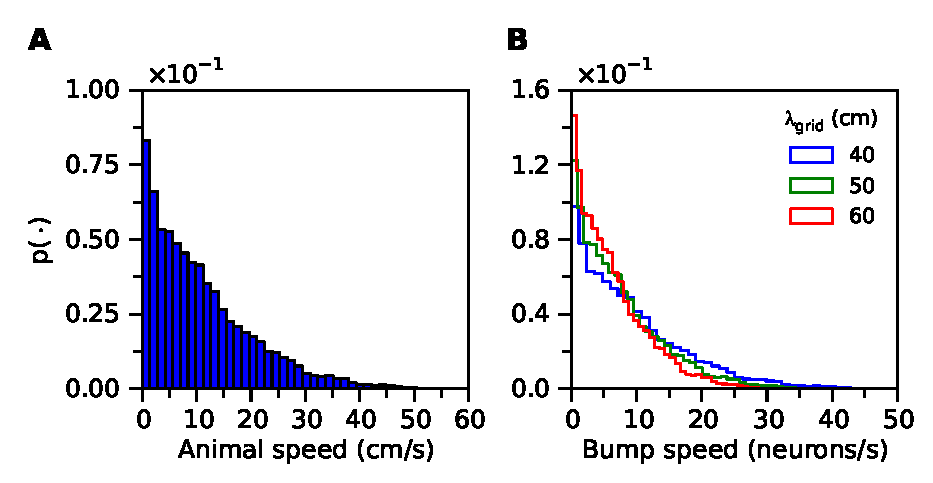
\includegraphics[trim=0 0.6cm 0 0 ]{fig/velocity_histograms}
    \end{center}
    \internallinenumbers
    \caption{\textbf{(A)} Histogram of velocities of a simulated animal.
    \textbf{(B)} Histogram of bump speeds derived from the animal velocities
    estimated in eq. \eqref{eq:bump_speeds}, for different grid field spacings.}
    \label{fig:velocity_histograms}
\end{figure}


\section{Simulation protocols} \label{sec:noise_protocols}

\subsection{Simulations of animal movement} \label{sec:noise_grids_protocol}

Simulations of animal movement were carried out for 600 seconds of simulated
time.  Here, for each value of $\gE$ and $\gI$, the main simulation run was
preceded by a number of shorter simulations which determined how much current
needs to be injected in order for the bump of activity to track the simulated
movement of an animal (Section~\ref{sec:gain_est}). This procedure calibrates
the gain of the velocity input current in order to produce grid fields with a
specified spacing between the peaks in the individual firing fields. The result
is a single number in units of neurons/s/pA, which determines the speed of the
bump as a function of injected velocity input. The spacing between the
individual fields of the grid firing fields was set to 60 cm in all of the
simulations.

During the main simulation run, the animal movement was simulated for 600 s.
Each of the runs was repeated 4 times for simulations in Fig.~2 and 3 times
for simulations in Fig.~6D-I and once for networks that contain additional
recurrent synapses between E cells or I cells, as well as in networks with
synapses generated probabilistically. These simulations use the estimated velocity
response gain in order to calibrate the spacing between the grid firing fields.
After the simulation was finished, a neuron in the bottom-left corner of the
torus was selected for analysis. For this cell the gridness score of its firing
field was computed. The reasoning behind choosing only a single cell to estimate
the gridness score is as follows. The grid firing fields in the network are a
result of coordination of activity of the network as a whole. If the network
forms a bump attractor that is able to accurately track animal movement, all
cells in the network will have grid-like firing fields that differ only in
their phases. On the other hand, if the bump attractor does not form, is
unstable, or does not accurately track the position of the animal, the gridness
score of all cells will be low.  Thus, the firing field of a single cell in the
network represents grid field computation in the network as a whole.  Moreover,
this cell can be selected arbitrarily. This condition might not hold in
simulations where I cells receive uncorrelated spatial inputs and therefore
firing fields of 100 randomly selected cells from both E and I populations were
used to calculate the gridness scores (Figure 2 -- figure
supplement~5).


\subsection{Short simulation runs without animal movement} \label{sec:noise_short_sims}

Some of the simulation runs were used to estimate properties of bump attractors
and nested gamma oscillations. 
In these experiments, instead of simulating animal movement, a shorter, ten
second simulation, was run. The velocity and place cell input were deactivated.
Thus, the network is expected to only produce a static bump attractor and does
not perform path integration. For each parameter setting (determined
by $\gE$, $\gI$, and the noise level), 5 simulations were performed.  For each
simulation run, post-synaptic currents were recorded from 25 randomly selected
excitatory cells in the model by clamping their membrane potential at
-50~mV (this was done by simulating a separate process for each of the selected
neurons, while simulating the original membrane potential according to
eq.~\eqref{eq:Vm}).
Thus, on each run, different cells could be
picked up for analysis. It is in principle possible to record membrane currents
from all the neurons. However, the amount of data generated by such simulations
quickly becomes overwhelming (on the order of several terabytes per
parameter exploration experiment). Thus the approach chosen here was to sample from
the population of neurons and store the recorded state variables of only a
subset of these. This allowed for unrestricted analysis and visualisation of
the recorded state variables.


\section{Analysis of nested gamma oscillations}

We have estimated the properties of nested gamma oscillations by using
autocorrelation functions of the inhibitory currents impinging from inhibitory
synapses onto excitatory cells. These currents have been estimated from 25
randomly selected excitatory cells recorded during the simulation run.  For
each neuron, the current was then band-pass filtered between 20 and 200 Hz, the
autocorrelation function was computed and then used to detect local maxima
after excluding the first peak. The positions of local maxima were calculated
as those points in the autocorrelation function where the first difference of
the signal changed sign from positive to negative and thus approximated points
where the first derivative is zero and the second derivative is negative.  The
power and frequency of the underlying oscillation was then estimated from the
correlation value and from the time lag of the first detected autocorrelation
peak respectively. Both values were averaged over all 25 recorded neurons and
then subsequently averaged over all simulation trials.

\section{Gaussian fitting procedure} \label{sec:gauss_fitting}

In networks where properties of bump attractors, such as the position and
presence of an activity bump, were estimated, we developed a procedure to fit
Gaussian functions onto successive snapshots of network activity of E cells.
The network activity snapshots were estimated by taking action potential times
of all E cells and estimating their immediate firing rate using a 250 ms wide
sliding window with a 125 ms time step. For each snapshot, the properties of a
bump-like network activity (if it was a bump) were then estimated by fitting a
symmetric Gaussian function to the network activity snapshots, using the
maximum likelihood estimator under Gaussian noise (the least squares
fitting method):
\begin{equation}
    B(\mathbf{X}) = A \exp\left(
        -\frac{||\mathbf{X} - \bm{\mu}||^2}{2\sigmasub{bump}^2} \right),
    \label{eq:noise_bump_fitting}
\end{equation}
where $A$ was the height of the Gaussian function, $\mathbf{X}$ was neuron position
on the twisted torus, $\bm{\mu}$ was the centre of the Gaussian,
$\sigmasub{bump}$ was the width of the Gaussian, and~$||\cdot||$ represents a
distance metric on the twisted torus. The parameters fitted were $A$,
$\bm{\mu}$ and $\sigmasub{bump}$. These parameters were then used as the basis
for further analysis.

\begin{table}
    \internallinenumbers
    \centering
    \begin{tabular}{| c | c | c | c |}
        \hline
        Name       & Units & Value (E cells) & Value (I cells) \\
        \hline\hline
        $\Cm$      & pF    & 211.389         & 227.3    \\
        $\EL$      & mV    & -68.5           & -60      \\
        $\VT$      & mV    & -50             & -45      \\
        $\Vr$      & mV    & -68.5           & -60      \\
        $\gL$      & nS    & 22.73           & 22.73    \\
        $\deltaT$  & mV    & 0.4             & 0.4      \\
        $\EAHP$    & mV    & -80             & $\times$ \\
        $\tauAHP$  & ms    & 20              & $\times$ \\
        $\gAHPmax$ & nS    & 5               & $\times$ \\
        $\tauad$   & ms    & $\times$        & 7.5      \\
        $\gadinc$  & nS    & $\times$        & 22.73    \\
        \hline
    \end{tabular}
    \caption{Single neuron parameter values for all cells.}
    \label{tab:params_E}
\end{table}

\begin{table}
    \internallinenumbers
    \centering
    \begin{tabular}{| c | c | c |}
        \hline
        Name       & Units & Value \\
        \hline\hline
        $\EAMPA$   & mV    & 0     \\
        $\tauAMPA$ & ms    & 1     \\
        $\ENMDA$   & mV    & 0     \\
        $\tauNMDA$ & ms    & 100   \\
        $\EGABAA$  & mV    & -75   \\
        $\tauGABAA$& ms    & 5     \\
        \hline
    \end{tabular}
    \caption{Parameter values for synapses.}
    \label{tab:params_synapses}
\end{table}

\begin{table}
    \internallinenumbers
    \centering
    \begin{tabular}{| c | c | c | c |}
        \hline
        Name       & Units & Value (E cells) & Value (I cells) \\
        \hline\hline
        $\Iconst$  & pA    & 300             & 200             \\
        $\Atheta$  & pA    & 375             & 25              \\
        $\phitheta$& rad   & $-\pi/2$        & $-\pi/2$        \\
        $\ftheta$  & Hz    & 8               & 8               \\
        \hline
    \end{tabular}
    \caption{Parameter values for external inputs.}
\end{table}

\begin{table}
    \internallinenumbers
    \centering
    \begin{tabular}{| c | c | c |}
        \hline
        Name              & Units                        & Value   \\
        \hline\hline
        $\mu$             & \multirow{4}{*}{normalised}  & 0.433   \\
        $\sigmasub{exc}$  &                              & 0.0834  \\
        $\sigmasub{inh}$  &                              & 0.0834  \\
        C                 &                              & 0.03    \\
        \lamgrid          & cm                           & 60      \\
        \hline
    \end{tabular}
    \caption{Parameter values for synaptic profiles.}
    \label{tab:params_syn}
\end{table}

\clearpage

\bibliographystyle{abbrv}
\bibliography{SupplementaryMethodsBib}


\clearpage

\section*{Figure Supplements}

\setcounter{figure}{0}
\makeatletter
\renewcommand{\fnum@figure}[1]{\textbf{\figurename~\thefigure}}
\makeatother
\renewcommand{\figurename}{Figure 1 - figure supplement}

\begin{figure}[h!]
    \internallinenumbers
    \centering
        \includegraphics{fig/output_figures/figure1S_weights.pdf}
    \raggedleft
    \caption{}
        %\caption{Synaptic weights in scaled and probabilistic variants of the
        %network. (A) Output (top) and input (bottom) synaptic weights of an E
        %(left) and I (right) neuron in the middle of the twisted torus in a
        %network in which synaptic weights are scaled according to the synaptic
        %profile functions from Figure 1B. (B) Same as (A), but synaptic weights
        %are constant and the probability of connection between a pair of
        %neurons is scaled according to the synaptic profile functions in
        %Figure~1B.}
\end{figure}

\clearpage


\begin{figure}[h!]
    \includegraphics[trim=0 0.5cm 0cm 0cm,width=\textwidth,center]{fig/panels/suppFigure_grid_examples_0}
\end{figure}

\clearpage


\newcounter{fnameCnt}
\setcounter{fnameCnt}{1}
\newcount\gridcnt
\gridcnt=1
\loop
    \def\gridfname{fig/panels/suppFigure_grid_examples_\arabic{fnameCnt}}
    \begin{figure}[t!]
        \begin{center}
       \includegraphics[trim=0cm 0.5cm 0cm 0cm, width=0.95\textwidth,center]
            {\gridfname}
        \end{center}
    \end{figure}
    \clearpage
    \stepcounter{fnameCnt}
    \advance \gridcnt 1
\ifnum \gridcnt<11
\repeat

\setcounter{figure}{0}
\renewcommand{\figurename}{Figure 2 - figure supplement}

\begin{figure}[h!]
    \includegraphics[trim=0 0.5cm 0cm 0cm,width=0.95\textwidth,center]{fig/panels/suppFigure_grid_examples_11}
    \caption{}
\end{figure}


%\begin{figure}[H]
%    \internallinenumbers
%    \contcaption{}
%    %\contcaption{Examples of spatial firing fields. (A-L) Top: Gridness score in
%    %the parameter space of the E and I synaptic strength scaling parameters
%    %($\gE$ and $\gI$ respectively). Bottom: Firing fields of a single cell
%    %obtained by simulating animal movement, in the parameter region highlighted
%    %by black rectangle in the parameter space plot. Above each firing field is
%    %the estimated gridness score (left) and maximal firing rate in the firing
%    %field (right). Blank (white) locations in the parameter space are
%    %simulations that did not finish in the pre-specified time limit (5 h).
%    %Noise level used in each set of simulations is shown by
%    %$\sigma_{\text{noise}}$. Color scale in the firing field plots ranges from
%    %0 Hz to the maximal firing rate for each of the firing fields.}
%\end{figure}

\clearpage

\begin{figure}[p]
    \internallinenumbers
    \centering
        \includegraphics[width=0.95\textwidth]{fig/output_figures/figure2S_prob_conn}
    \caption{}
    %\caption{
    %Sensitivity of grid firing to changes in feedback inhibition, excitation and noise
    %levels in networks with connection probability between pairs of neurons drawn
    %according to the synaptic profile functions in Figure 1B. 
    %(A-C) Example spatial firing fields (left) and spatial autocorrelation plots
    %(right) of E and I cells for networks without noise (A; $\sigma$ = 0 pA), with noise
    %set to $\sigma$ = 150 pA (B), and noise set to $\sigma$ = 300 pA (C) and with the
    %strengths of recurrent synaptic connections indicated by arrows in (D-F).
    %Maximal firing rate is indicated in the top right of each spatial firing plot.
    %The range of spatial autocorrelations is normalized between 0 and 1. (D-F)
    %Gridness score as a function of gE and gI for networks with each noise level.
    %Each item in the color plot is an average gridness score of two simulation
    %runs. Arrows indicate the positions of grid field and autocorrelation examples
    %from simulations illustrated in (A-C). Simulations that did not finish in a
    %specified time interval (5 h) are indicated by white color.}
    %\label{fig:grids_prob_conn}
\end{figure}

\clearpage

\begin{figure}[p]
    \internallinenumbers
    \centering
        \includegraphics[width=0.95\textwidth]{fig/output_figures/figure2S_default_info_scores}
    \caption{}
\end{figure}

\clearpage

%\begin{figure}[H]
%    \internallinenumbers
%    \caption{Spatial information and sparsity of firing fields of E and I
%    cells. (A) Spatial information of E (top) and I (bottom) cells as a
%    function of $\gE$ and $\gI$ in networks from Figure 2. (B) Same as (A), but
%    the color plots show spatial sparsity of E and I cells. Black lines
%    indicate the region from Figure 2D-F where the gridness score = 0.5.}
%\end{figure}
%
%\clearpage

\begin{figure}[p]
    \internallinenumbers
    \centering
        \includegraphics[width=0.95\textwidth]{fig/output_figures/figure2S_default_i_fields}
    \caption{}
    %\caption{Gridness scores of I cells as a function of $\gE$ and $\gI$ for
    %networks without noise (A), with noise standard deviation $\sigma$ = 150
    %pA (B), and $\sigma$ = 300 pA (C). Data are from simulations of networks
    %with feedback inhibition only (E-I networks; Figure 2). Black lines
    %indicate the region from Figure 2D-F where the gridness score of E cells = 0.5.}
\end{figure}

\clearpage

%\begin{figure}[p]
%    \internallinenumbers
%    \centering
%        \includegraphics[width=0.95\textwidth]{fig/output_figures/figure2S_prob_conn_i_fields}
%    \caption{Firing fields and gridness scoress of I cells in networks with
%    connection probability between pairs of neurons drawn according to the
%    synaptic profile functions in Figure 1B (A-C) Example firing fields (left)
%    and spatial autocorrelation plots (right) for the specific values of
%    strengths of recurrent synaptic connections indicated by arrows in (D-F),
%    corresponding to the three simulated noise levels.  (D-F) Gridness score as
%    a function of $\gE$ and $\gI$ for networks without noise (D; $\sigma$ = 0
%    pA), with noise level set to $\sigma$ = 150 pA (E), and noise level set to
%    $\sigma$ = 300 pA (F). Arrows indicate the positions of grid field and
%    autocorrelation examples from simulations illustrated in (A-C). Simulations
%    that did not finish in a specified time interval (8 h) are indicated by
%    white color.}
%\end{figure}
%
%\clearpage

\begin{figure}[p]
    \internallinenumbers
    \centering
        \includegraphics[width=0.95\textwidth]{fig/output_figures/figure2S_i_place_cells}
    \caption{}
    %\caption{Spatial firing fields in networks with uncorrelated spatial input
    %applied to each I cell. Each I cell received connections from 3 randomly
    %selected neurons with a place like spatial firing field.  (A) Examples of
    %firing fields of E and I cells. Gridness score and maximal firing rate of
    %the firing field is indicated in the top left and right parts of each
    %firing field, respectively. (B) Distributions of spatial sparsity (left),
    %spatial information (centre) and gridness score (right) of 100 randomly
    %selected cells from each population of neurons. Each simulation run was
    %repeated 10 times with different randomisation seeds. Properties of place
    %cells: \ssc{r}{max}{}~=~100 Hz, \ssc{\sigma}{field}{}~=~80 cm. Network
    %parameters were $\gE$ = 3 nS and $\gI$ = 1 nS.}
    %\label{fig:ipc}
\end{figure}

\clearpage

%\begin{figure}[p]
%    \internallinenumbers
%    \centering
%        \includegraphics[width=0.95\textwidth]{fig/output_figures/figure2S_i_surround}
%    \caption{\todo[inline]{Grids in I-surround networks.}}
%\end{figure}
%
%\clearpage

\setcounter{figure}{0}
\renewcommand{\figurename}{Figure 3 - figure supplement}

\begin{figure}[p]
    \internallinenumbers
    \centering
        \includegraphics{fig/output_figures/figure3S_prob_conn}
    \caption{}
\end{figure}

\clearpage

%\begin{figure}[H]
%    \internallinenumbers
%    \caption{Sensitivity of gamma oscillations to changes in the strength of E
%    and I synapses in networks with connection probability between pairs of
%    neurons drawn according to the synaptic profile functions in Figure 1B.
%    (A-C) Examples of inhibitory (red) and excitatory (blue) synaptic currents
%    recorded respectively from excitatory and inhibitory neurons from
%    simulations highlighted by arrows in panels (D-F).  (D-F) Top: Correlation
%    value at the first local maximum of an autocorrelation of inhibitory
%    synaptic currents (I$\rightarrow$E cells, 25 randomly selected E cells),
%    plotted as a function of $\gE$ and $\gI$, for networks without noise (D), with
%    noise set to $\sigma$ = 150 pA (E), and noise set to $\sigma$ =
%    300 pA (F). Each point is an average over five simulation trials. In these
%    simulations velocity and place cell inputs were disabled.  The duration of
%    simulations was 10 seconds.  Bottom: Frequency corresponding to the peaks
%    of the autocorrelation functions for simulations in the top panels. Black
%    lines in (E) indicate the region from Figure 2 - figure
%    supplement~\ref{fig:grids_prob_conn} where the gridness score = 0.5}
%\end{figure}
%
%\clearpage

%\begin{figure}[p]
%    \internallinenumbers
%    \centering
%        %\includegraphics{fig/output_figures/figure3S_i_surround}
%    \caption{\todo[inline]{I-surround simulations will go here.}}
%\end{figure}
%
%\clearpage
%
%\begin{figure}[H]
%    \internallinenumbers
%    \caption{Sensitivity of gamma oscillations to changes in the strength of E
%    and I synapses in networks in the I-surround configuration (cf.\
%    \cite{Pastoll:2013ff}).  (A-C) Examples of inhibitory (red) and excitatory
%    (blue) synaptic currents recorded respectively from excitatory and
%    inhibitory neurons from simulations highlighted by arrows in panels (D-F).
%    (D-F) Top: Correlation value at the first local maximum of an
%    autocorrelation of inhibitory synaptic currents (I$\rightarrow$E cells, 25
%    randomly selected E cells), plotted as a function of $\gE$ and $\gI$, for
%    networks without noise (D), with noise level set to $\sigma$ = 150 pA (E),
%    and noise level set to $\sigma$ = 300 pA (F). Each point is an average over
%    five simulation trials. In these simulations velocity and place cell inputs
%    were disabled.  The duration of simulations was 10 seconds.  Bottom:
%    Frequency corresponding to the peaks of the autocorrelation functions for
%    simulations in the top panels.}
%\end{figure}
%
%\clearpage

\begin{figure}[p]
    \internallinenumbers
    \centering
        \includegraphics[trim=0 0.5cm 0cm 0cm]{fig/panels/suppFigure_gamma.pdf}
    \caption{}
\end{figure}

\clearpage

\begin{figure}[ht!]
    \internallinenumbers
    \centering
        \includegraphics{fig/panels/suppFigure_gammaF_grids_scatter.pdf}
    \caption{}
\end{figure}

\clearpage

\begin{figure}[p]
    \internallinenumbers
    \centering
        \includegraphics{fig/output_figures/Figure3_S4}
    \caption{}
\end{figure}

\clearpage

%\setcounter{figure}{0}
%\renewcommand{\figurename}{Figure 4 - figure supplement}
%
%\begin{figure}[p]
%    \internallinenumbers
%    \centering
%        \includegraphics[width=0.95\textwidth]{fig/output_figures/figure4S_prob_conn}
%    \caption{Continuous attractors in networks with connection probability
%    between pairs of neurons drawn according to the synaptic profile functions
%    in Figure 1B. (A) Examples of E cell population firing rate snapshots from
%    simulations in which velocity and place cell inputs are inactivated. Each
%    row shows a simulation trial with a value of $\gE$ and $\gI$ highlighted by an
%    arrow in panel (B). The corresponding probability of bump formation
%    (P(bumps)) is indicated to the left.  (B) Color plots show probability of
%    bump formation (P(bumps)), for the simulated range of $\gE$ and $\gI$ and the
%    three simulated noise levels. Each color point is an average of five 10 s
%    simulation runs. Arrows show positions in the parameter space of examples
%    in (A).}
%\end{figure}
%
%\clearpage
%
%\begin{figure}[p]
%    \internallinenumbers
%    \centering
%        %\includegraphics[width=0.95\textwidth]{fig/output_figures/figure4S_i_surround}
%    \caption{\todo[inline]{Put here I-surround attractor simulations if we use
%    them.}}
%    %\caption{Continuous attractors in networks in the I-surround configuration
%    %(cf.\ \cite{Pastoll:2013ff}). (A) Examples of E cell population firing rate
%    %snapshots from simulations in which velocity and place cell inputs are
%    %inactivated. Each row shows a simulation trial with a value of $\gE$ and
%    %$\gI$
%    %highlighted by an arrow in panel (B). The corresponding probability of bump
%    %formation (P(bumps)) is indicated to the left.  (B) Color plots show
%    %probability of bump formation (P(bumps)), for the simulated range of $\gE$ and
%    %$\gI$ and the three simulated noise levels. Each color point is an average of
%    %five 10 s simulation runs. Arrows show positions in the parameter space of
%    %examples in (A).}
%\end{figure}
%
%\clearpage

\begin{figure}[p]
    \centering
        \includegraphics{fig/panels/raster_examples_0.pdf}
\end{figure}

\begin{figure}[p]
    \centering
        \includegraphics{fig/panels/raster_examples_1.pdf}
\end{figure}

\setcounter{figure}{0}
\renewcommand{\figurename}{Figure 5 - figure supplement}

\begin{figure}[p]
    \centering
        \includegraphics[trim=0 1cm 0 0]{fig/panels/raster_examples_2.pdf}
    \caption{}
\end{figure}

\clearpage

%\begin{figure}[p]
%    \internallinenumbers
%    \centering
%        \includegraphics[width=\textwidth]{fig/output_figures/figure5S_prob_conn}
%\end{figure}
%
%\clearpage
%
%\begin{figure}[H]
%    \internallinenumbers
%    \caption{Seizure-like states in networks with connection probability
%    between pairs of neurons drawn according to the synaptic profile functions
%    in Figure 1B. (A-C) Raster plots show activity of all neurons in the
%    excitatory (red) and inhibitory (blue) populations for the duration of two
%    theta cycles (top), along with the average population firing rates for both
%    populations (center and bottom; calculated with a sliding rectangular
%    window with 2 ms duration and 0.5 ms time step), for networks where noise
%    is absent (A; $\sigma$ = 0), with noise set to $\sigma$ = 150 pA (B), and
%    with noise set to $\sigma$ = 300 pA (C). Simulations were performed in the
%    absence of animal movement and place cell input; $\gE$ = 1 nS and $\gI$ = 3 nS.
%    (D) Maximal average population firing rate of E cells estimated from the
%    whole simulation run (10 s; 500 ms at the beginning of the simulation
%    excluded) for each simulated level of noise. Each point is an average of
%    maxima from 5 simulation runs.  (E) Probability of the maximal
%    population-average firing rate during each theta cycle exceeding 300 Hz,
%    i.e. at least 60\% of E cells firing synchronously within a time period of
%    2 ms in the parameter space of $\gE$ and $\gI$. Black lines indicate regions
%    where gridness score equals 0.5.
%    (F) Scatter plots show the relationship between gridness score and the
%    maximal firing rate during the simulation (left) and the probability of the
%    maximal population-average firing rate during each theta cycle exceeding
%    300 Hz (right).}
%\end{figure}
%
%\clearpage
%
%\begin{figure}[p]
%    \internallinenumbers
%    \centering
%        \includegraphics[width=0.95\textwidth]{fig/output_figures/figure5S_i_surround}
%\end{figure}
%
%\clearpage
%
%\begin{figure}[H]
%    \internallinenumbers
%    \caption{Seizure-like states in networks in the I-surround configuration
%    (cf. \cite{Pastoll:2013ff}). (A-C) Raster plots show activity of all
%    neurons in the excitatory (red) and inhibitory (blue) populations for the
%    duration of two theta cycles (top), along with the average population
%    firing rates for both populations (center and bottom; calculated with a
%    sliding rectangular window with 2 ms duration and 0.5 ms time step), for
%    networks where noise is absent (A; $\sigma$ = 0), with noise set to
%    $\sigma$ = 150 pA (B), and with noise set to $\sigma$ = 300 pA (C).
%    Simulations were performed in the absence of animal movement and place cell
%    input; $\gE$ = 1 nS and $\gI$ = 3 nS.  (D) Maximal average population firing rate
%    of E cells estimated from the whole simulation run (10 s; 500 ms at the
%    beginning of the simulation excluded) for each simulated level of noise.
%    Each point is an average of maxima from 5 simulation runs.  (E) Probability
%    of the maximal population-average firing rate during each theta cycle
%    exceeding 300 Hz, i.e. at least 60\% of E cells firing synchronously within
%    a time period of 2 ms in the parameter space of $\gE$ and $\gI$. Black lines
%    indicate regions where gridness score equals 0.5.}
%\end{figure}
%
%\clearpage


\setcounter{figure}{0}
\renewcommand{\figurename}{Figure 6 - figure supplement}

\begin{figure}[ht!]
    \internallinenumbers
    \centering
        \includegraphics{fig/output_figures/Figure6_S1}
    \caption{}
\end{figure}

\clearpage

\begin{figure}[ht!]
    \internallinenumbers
    \centering
        \includegraphics{fig/output_figures/Figure6_S2}
    \caption{}
\end{figure}

\clearpage

\begin{figure}[ht!]
    \internallinenumbers
    \centering
        \includegraphics{fig/output_figures/Figure6_S3}
    \caption{}
\end{figure}

\clearpage

\begin{figure}[ht!]
    \internallinenumbers
    \centering
        \includegraphics[center]{fig/output_figures/Figure6_S4}
    \caption{}
\end{figure}

\clearpage

\begin{figure}[ht!]
    \internallinenumbers
    \centering
        \includegraphics{fig/output_figures/Figure6_S5}
    \caption{}
\end{figure}

\clearpage

\begin{figure}[ht!]
    \internallinenumbers
    \centering
        \includegraphics{fig/output_figures/Figure6_S6}
    \caption{}
\end{figure}

\clearpage

%\begin{figure}[ht!]
%    \internallinenumbers
%    \centering
%        \includegraphics[center]{fig/output_figures/figure6S_prob_conn}
%    \caption{Calibration of the gain of the velocity inputs in networks with
%    connection probability between pairs of neurons drawn according to the
%    synaptic profile functions in Figure 1B. (A-C) Bump attractor speed as a
%    function of the strength of the velocity current for the three simulated
%    levels of noise. Ten simulation runs were performed for each level of noise
%    (blue markers). In each run the speed of the bump was calculated in
%    response to the injected velocity input and the data were used to fit a
%    linear relationship using an estimation procedure outlined in Supplementary
%    Methods (black line). (D-F) Slope of the estimated velocity gain of the
%    attractor networks as a function of $\gE$ and $\gI$ for all simulated
%    levels of noise. (G-I) Same as in (D-F) but the plots show error of fit for
%    the estimated linear relationships. Arrows show locations of the data
%    plotted in (A-C).}
%\end{figure}
%
%\clearpage
%
%\begin{figure}[ht!]
%    \internallinenumbers
%    \centering
%        \includegraphics{fig/output_figures/figure6S_drift_prob_conn}
%    \caption{Sensitivity of bump attractor spontaneous drift to variations in
%    $\gE$ and $\gI$ and noise levels in networks with connections probability
%    between pairs of neurons drawn according to the synaptic profile functions
%    in Figure 1B. (A) Schematic of the bump attractor drift estimation
%    procedure. The first 500 ms of a simulation trial are used to initialise
%    the bump attractor. Onset of theta modulated input current was at 500 ms.
%    The estimated centres of bump attractors measured by the least squares fit
%    of symmetric Gaussians were at 1 s (initial position) and 9 s (final
%    position). The drift was then estimated as the distance on twisted torus
%    between the initial and final position. Simulation time was 10 s. (B)
%    Colour plots show bump attractor drifts averaged over 5 simulation trials,
%    for the simulated ranges of excitatory and inhibitory synaptic strengths
%    and levels of noise.  Networks without noise can form stable bump
%    attractors in a subset of their parameter region. Networks with noise
%    suffer from attractor drift in majority of the parameter region. Black
%    contours show isoclines of gridness score equal to 0.5.}
%\end{figure}
%
%\clearpage
%
%\begin{figure}[ht!]
%    \internallinenumbers
%    \centering
%        \includegraphics[center]{fig/output_figures/figure6S_i_surround}
%    \caption{Calibration of the gain of the velocity inputs in networks in the
%    I-surround configuration (cf. \cite{Pastoll:2013ff}). (A-C) Bump attractor
%    speed as a function of the strength of the velocity current for the three
%    simulated levels of noise. Ten simulation runs were performed for each
%    level of noise (blue markers). In each run the speed of the bump was
%    calculated in response to the injected velocity input and the data were
%    used to fit a linear relationship using an estimation procedure outlined in
%    Supplementary Methods (black line). (D-F) Slope of the estimated velocity
%    gain of the attractor networks as a function of $\gE$ and $\gI$ for all
%    simulated levels of noise. (G-I) Same as in (D-F) but the plots show error
%    of fit for the estimated linear relationships. Arrows show locations of the
%    data plotted in (A-C).
%    \todo[inline]{This doesn't look as good as I though. The slope in 150pA
%    case is rather shallow and the error higher. We should however wait for the
%    grid field simulations first.}}
%\end{figure}
%
%\clearpage

%\begin{figure}[ht!]
%    \internallinenumbers
%    \centering
%        \includegraphics{fig/output_figures/figure6S_drift_i_surround}
%    \caption{Sensitivity of bump attractor spontaneous drift to variations in
%    $\gE$ and $\gI$ and noise levels in networks in the I-surround
%    configuration (cf. \cite{Pastoll:2013ff}). (A) Schematic of the bump
%    attractor drift estimation procedure. The first 500 ms of a simulation
%    trial are used to initialise the bump attractor. Onset of theta modulated
%    input current was at 500 ms.  The estimated centres of bump attractors
%    measured by the least squares fit of symmetric Gaussians were at 1 s
%    (initial position) and 9 s (final position). The drift was then estimated
%    as the distance on twisted torus between the initial and final position.
%    Simulation time was 10 s. (B) Colour plots show bump attractor drifts
%    averaged over 5 simulation trials, for the simulated ranges of excitatory
%    and inhibitory synaptic strengths and levels of noise.  Networks without
%    noise can form stable bump attractors in a subset of their parameter
%    region. Networks with noise suffer from attractor drift in majority of the
%    parameter region. Black contours show isoclines of gridness score equal to
%    0.5.}
%\end{figure}
%
%\clearpage

\setcounter{figure}{0}
\renewcommand{\figurename}{Figure 7 - figure supplement}


\begin{figure}[p]
    \internallinenumbers
    \centering
        \includegraphics[width=0.95\textwidth]{fig/output_figures/figure7S_grids_examples}
    \caption{}
\end{figure}

\clearpage

\begin{figure}[p]
    \internallinenumbers
    \centering
        \includegraphics[width=0.95\textwidth]{fig/output_figures/figure7S_bumps}
    \caption{}
\end{figure}

\clearpage

\begin{figure}[ht!]
    \internallinenumbers
    \centering
        \includegraphics{fig/output_figures/figure7S_drift}
    \caption{}
\end{figure}

\clearpage

\begin{figure}[ht!]
    \internallinenumbers
    \centering
        \includegraphics[center]{fig/output_figures/figure7S_velocity}
    \caption{}
\end{figure}

\clearpage

\begin{figure}[p]
    \internallinenumbers
    \centering
        \includegraphics[width=\textwidth]{fig/output_figures/figure7S_seizures}
    \caption{}
\end{figure}

\clearpage

\begin{figure}[p]
    \internallinenumbers
    \centering
        \includegraphics[width=0.95\textwidth]{fig/output_figures/Figure7_S6}
    \caption{}
\end{figure}

\clearpage

\begin{figure}[p]
    \internallinenumbers
    \centering
        \includegraphics{fig/output_figures/Figure7_S7}
    \caption{}
\end{figure}

\clearpage

\begin{figure}[p]
    \internallinenumbers
    \centering
        \includegraphics[width=0.95\textwidth]{fig/output_figures/Figure7_S8}
    \caption{}
\end{figure}

\clearpage

\begin{figure}[p]
    \internallinenumbers
    \centering
        \includegraphics[width=0.95\textwidth]{fig/output_figures/Figure7_S9}
    \caption{}
\end{figure}

\clearpage

%\begin{figure}[ht!]
%    \internallinenumbers
%    \centering
%        \includegraphics{fig/output_figures/figure6S_drift_ee_connections}
%    \caption{Sensitivity of bump attractor spontaneous drift to variations in
%    $\gE$ and $\gI$ and noise levels in networks that contain direct
%    E$\rightarrow$E synapses. (A) Schematic of the bump attractor drift
%    estimation procedure. The first 500 ms of a simulation trial are used to
%    initialise the bump attractor. Onset of theta modulated input current was
%    at 500 ms.  The estimated centres of bump attractors measured by the least
%    squares fit of symmetric Gaussians were at 1 s (initial position) and 9 s
%    (final position). The drift was then estimated as the distance on twisted
%    torus between the initial and final position. Simulation time was 10 s. (B)
%    Colour plots show bump attractor drifts averaged over 5 simulation trials,
%    for the simulated ranges of excitatory and inhibitory synaptic strengths
%    and levels of noise.  Networks without noise can form stable bump
%    attractors in a subset of their parameter region. Networks with noise
%    suffer from attractor drift in majority of the parameter region. Black
%    contours show isoclines of gridness score equal to 0.5.}
%\end{figure}
%
%\clearpage
%
%\begin{figure}[ht!]
%    \internallinenumbers
%    \centering
%        \includegraphics[center]{fig/output_figures/figure6S_ee_connections}
%    \caption{Calibration of the gain of the velocity inputs in networks that
%    contain direct E$\rightarrow$E synapses. (A-C) Bump attractor speed as a
%    function of the strength of the velocity current for the three simulated
%    levels of noise. Ten simulation runs were performed for each level of noise
%    (blue markers). In each run the speed of the bump was calculated in
%    response to the injected velocity input and the data were used to fit a
%    linear relationship using an estimation procedure outlined in Supplementary
%    Methods (black line). (D-F) Slope of the estimated velocity gain of the
%    attractor networks as a function of $\gE$ and $\gI$ for all simulated
%    levels of noise. (G-I) Same as in (D-F) but the plots show error of fit for
%    the estimated linear relationships. Arrows show locations of the data
%    plotted in (A-C).}
%\end{figure}
%
%\clearpage

\begin{figure}[p!]
    \internallinenumbers
    \centering
        \includegraphics[width=0.95\textwidth]{fig/output_figures/figure7S_ee_ei_flat_networks_0}
\end{figure}

\clearpage

\begin{figure}[p!]
    \internallinenumbers
    \centering
        \includegraphics[width=0.95\textwidth]{fig/output_figures/figure7S_ee_ei_flat_networks_1}
\end{figure}

\begin{figure}[p!]
    \internallinenumbers
    \centering
        \includegraphics[width=0.95\textwidth]{fig/output_figures/figure7S_ee_ei_flat_networks_2}
    \caption{}
\end{figure}

\end{document}

